\doc{La balance \textsc{METTLER} P1200}

% METTLER ou METLER ?

\pagestyle{empty}


\vressort{3}

\begin{Large}
\hressort{1}
\emph{Port�e :} $1200~g$
\hressort{3}
\emph{Sensibilit� : } $0,01~g$
\hressort{1}
\end{Large}

\vressort{3}

\begin{center}
\includegraphics{thermodynamique/doc_balance_metler_p1200/balance_mettler.eps}
\caption{Sch�ma de la balance}
\end{center}

\vressort{3}


\begin{enumerate}
\item V�rifier l'horizontalit� de la balance (vis de calage + bulle B

\item Allumer. La balance doit �tre � $000,00~g$. L'�l�ve pr�cedent
  doit l'y avoir mise (sinon l'y mettre). Le bouton de tarage doit
  �tre lui aussi � z�ro ( en but�e)

\item Si pes�e directe d'un r�cipient R

  \begin{enumerate}
    \item Poser d�licatement R sur le plateau

    \item Si �chelle lumineuse d�pass�e (le signe + appara�t),
      abaisser d�licatement les centaines de $g$ n�cessaires.

    \item R�gler les centi�mes de $g$

    \item Relever  $m = \Box\Box\Box,\Box\Box~g$

   \end{enumerate}

  \item Si pes�e d'une poudre ou d'un liquide :

   \begin{enumerate}
     \item Tarer le r�cipient R :
       \begin{itemize}
         \item le poser (vide) sur le plateau
         \item tarer � z�ro (bouton TARA $0-100$ + molette de tarage
           fin)


           \emph{NE PLUS TOUCHER AU TARRAGE PENDANT LA PES\'EE}

       \end{itemize}

     \item Avec spatule verser les cristaux jusqu'� masse de
       poudre d�sir�e (ou verser le liquide)

     \item R�gler les centi�mes de $g$.
       
     \item Relever $m = \Box\Box\Box,\Box\Box~g$

   \end{enumerate}

\item \'Eteindre la balance. Enlever le r�cipient du plateua. Rallumer
  et mettre tout � z�ro (bouton de tarage ; centaines de $g$ ;
  centi�me de $g$)
   

\end{enumerate}

